
\documentclass[12pt,letterpaper,noanswers]{exam}
\usepackage[usenames,dvipsnames,svgnames,table]{xcolor}
\usepackage[margin=0.9in]{geometry}
\renewcommand{\familydefault}{\sfdefault}
\usepackage{multicol}
\pagestyle{head}
\header{AM 111 Class 04}{}{Linear least squares, p.\thepage}
\runningheadrule
\headrule
\usepackage{siunitx}
\usepackage{enumitem}
\usepackage{graphicx} % more modern
\usepackage{amsmath} 
\usepackage{amssymb} 
\usepackage{hyperref}

\usepackage[most]{tcolorbox}
\usepackage{listings}

\definecolor{white}{rgb}{1,1,1}
\definecolor{mygreen}{rgb}{0,0.4,0}
\definecolor{light_gray}{rgb}{0.97,0.97,0.97}
\definecolor{mykey}{rgb}{0.117,0.403,0.713}

\tcbuselibrary{listings}
\newlength\inwd
\setlength\inwd{1.3cm}
% https://tex.stackexchange.com/questions/340700/ipython-notebook-input-and-output-cells-with-listings
\newcounter{ipythcntr}
\renewcommand{\theipythcntr}{\texttt{[\arabic{ipythcntr}]}}

\newtcblisting{pyin}[1][]{%
  sharp corners,
  enlarge left by=\inwd,
  width=\linewidth-\inwd,
  enhanced,
  boxrule=0pt,
  colback=light_gray,
  listing only,
  top=0pt,
  bottom=0pt,
  overlay={
    \node[
      anchor=north east,
      text width=\inwd,
      font=\footnotesize\ttfamily\color{mykey},
      inner ysep=2mm,
      inner xsep=0pt,
      outer sep=0pt
      ] 
      at (frame.north west)
      {\refstepcounter{ipythcntr}\label{#1}In \theipythcntr:};
  }
  listing engine=listing,
  listing options={
    aboveskip=1pt,
    belowskip=1pt,
    basicstyle=\footnotesize\ttfamily,
    language=Python,
    keywordstyle=\color{mykey},
    showstringspaces=false,
    stringstyle=\color{mygreen}
  },
}
\newtcblisting{pyprint}{
  sharp corners,
  enlarge left by=\inwd,
  width=\linewidth-\inwd,
  enhanced,
  boxrule=0pt,
  colback=white,
  listing only,
  top=0pt,
  bottom=0pt,
  overlay={
    \node[
      anchor=north east,
      text width=\inwd,
      font=\footnotesize\ttfamily\color{mykey},
      inner ysep=2mm,
      inner xsep=0pt,
      outer sep=0pt
      ] 
      at (frame.north west)
      {};
  }
  listing engine=listing,
  listing options={
      aboveskip=1pt,
      belowskip=1pt,
      basicstyle=\footnotesize\ttfamily,
      language=Python,
      keywordstyle=\color{mykey},
      showstringspaces=false,
      stringstyle=\color{mygreen}
    },
}
\newtcblisting{pyout}[1][\theipythcntr]{
  sharp corners,
  enlarge left by=\inwd,
  width=\linewidth-\inwd,
  enhanced,
  boxrule=0pt,
  colback=white,
  listing only,
  top=0pt,
  bottom=0pt,
  overlay={
    \node[
      anchor=north east,
      text width=\inwd,
      font=\footnotesize\ttfamily\color{mykey},
      inner ysep=2mm,
      inner xsep=0pt,
      outer sep=0pt
      ] 
      at (frame.north west)
      {\setcounter{ipythcntr}{\value{ipythcntr}}Out#1:};
  }
  listing engine=listing,
  listing options={
      aboveskip=1pt,
      belowskip=1pt,
      basicstyle=\footnotesize\ttfamily,
      language=Python,
      keywordstyle=\color{mykey},
      showstringspaces=false,
      stringstyle=\color{mygreen}
    },
}





\newcommand{\note}[1]{\textcolor{red}{#1}} % show notes in red
\renewcommand{\note}[1]{} % don't display notes

\begin{document}
 \pdfpageheight 11in 
  \pdfpagewidth 8.5in

\noindent 

\note{calendar:
\begin{enumerate}
    \item Tu binary subtraction, least sq intro PS01/2
    \item Th least sq PS02
    \item Tu lin alg PS02/3
    \item Th lin alg PS03
    \item Tu least sq PS03/4
    \item Th ?? PS04
    \item Tu root finding PS04/5
    \item Th root finding PS05 (early)
    \item Tu integration PS06
    \item Th quiz
    \item Tu interpolation PS06
    \item Th interpolation PS06
    \item Tu integration PS07
    \item Th Monte Carlo PS07
    \item Tu differentiation PS08
    \item Th differentiation PS08
    \item Tu diff eq
    \item Th application of diff eq
    \item Tu ODEs
    \item Th ODEs
    \item Tu neural nets
    \item Tu neural nets
    \item Th quiz
    \item Tu presentations
\end{enumerate}}

\note{
\begin{itemize}
    \item what is a floating point system
    \item example
    \item IDing info about a floating point system
    \item 
\end{itemize}
}
\setcounter{section}{-1}
\section{Preliminaries}
\begin{itemize}
\itemsep0pt
\item There will be a skill check in class during the next class.  The problem info is below.
\item Problem set 01 is due on Friday.
\item Labs and OH.
\end{itemize}

\hrule
\vspace{0.2cm}


\noindent\textbf{Big picture}
\begin{itemize}
    \itemsep0pt
\item How do we solve a linear least squares problem?
\item How do we measure the sensitivity of a problem to small errors?
\end{itemize}

\vspace{0.2cm}
\hrule
\vspace{0.2cm}

\noindent \textbf{Skill check practice}

Set up a model, written in matrix form, for finding a parabola, $y = c_1 + c_2 t + c_2 t^2$, through the data points $(-1,1), (0,0)$, $(1,0), (2,-2)$.

\emph{Do not create the normal equations.}



\vspace{0.2cm}
\hrule
\vspace{0.2cm}

\noindent \textbf{Skill check solution}

The $y$ values go on the right hand side.  On the left hand side, the $A$ matrix has columns $1$, $t$, $t^2$.  The unknown coefficients are $c_1, c_2, c_3$.

$\left[\begin{array}{c c c}1 & -1 & 1 \\
1 & 0 & 0 \\
1 & 1 & 1 \\
1 & 2 & 4\end{array}\right]\left[\begin{array}{c}c_1\\c_2\\c_3\end{array} \right]= \left[\begin{array}{c}1 \\ 0 \\ 0 \\ -2\end{array}\right]$


\vspace{0.2cm}
\hrule
\vspace{0.2cm}

\section{Lower dimensional representations}
\subsection{Cost functions}
Using different cost functions leads to different choices of parameters to minimize the cost.

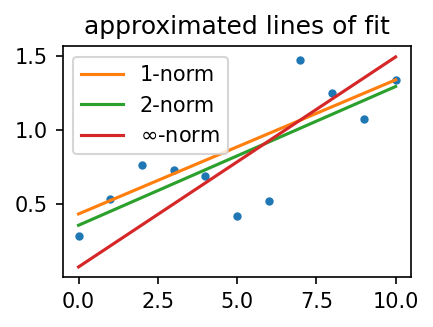
\includegraphics{AM111-F23-CourseNotes/img/c04-line.png}

\begin{enumerate}
\item Based on the Python code that was used to generate this figure (shared via projector), what was the method for finding the coefficients of each best fit line?
\item Will that method yield the linear least squares solution when the $2$-norm is used?  Why or why not?
\end{enumerate}

\begin{tcolorbox}
(directly from Greenbaum and Chartier, \S7.4.1) 

What is a norm?

A \textbf{norm} for vectors is a function $\Vert \cdot \Vert$ satisfying, for all $m$-vectors $\mathbf{u},\mathbf{w}$
\begin{enumerate}
\itemsep0pt
    \item $\Vert \mathbf{v}\Vert \geq 0$, with $\Vert \mathbf{v}\Vert = 0$ if and only if $\mathbf{v} = \mathbf{0}$
    \item $\Vert \alpha \mathbf{v} \Vert= \vert \alpha\vert\Vert\mathbf{v}\Vert$ for any scalar $\alpha$
    \item $\Vert \mathbf{v}+\mathbf{w}\Vert\leq \Vert\mathbf{v}\Vert+\Vert\mathbf{w}\Vert$ (triangle inequality)
\end{enumerate}
\end{tcolorbox}


\begin{enumerate}[resume]
\item In the $x_1x_2$-plane, let  $\mathbf{v}=(x_1,x_2)$.  
\begin{parts}
\item Set up an equation describing the set of points in the plane so that $\Vert\mathbf{v}\Vert_2 = 1$ (and sketch the set of points).
\item Set up one or more equations describing the set of points in the plane so that $\Vert\mathbf{v}\Vert_1 = 1$  (and sketch the set of points).
\item Set up one or more equations describing the set of points in the plane so that $\Vert\mathbf{v}\Vert_{\infty} = 1$  (and sketch the set of points).
\end{parts}

\end{enumerate}


\section{Linear least squares}





\subsection{Definitions}
\begin{tcolorbox}
\begin{itemize}
\itemsep0pt
    \item The term \textbf{least squares} refers to the choice of the $2$-norm as the cost-function.
    \item The function fitting problem is linear when the model, $f(x)$, can be expressed as a linear combination of functions $\varphi_k(x)$ where the functions are linearly independent.
    
    $\displaystyle f(x; \mathbf{c}) = \sum\limits_{i=1}^M c_k \varphi_k(x)$
    
    where $\mathbf{c} = (c_1,...c_M)$ are unknown weights.
    \item The functions $\varphi_k(x)$ are called \textbf{basis functions}.
    \item The \textbf{linear least squares} method refers to a model that is linear in the parameters $\mathbf{c}$ and is fit to data by minimizing a sum of squared error cost function.
    
    \[\text{Error}(\mathbf{c}) = \Vert \mathbf{e}(\vec{c})\Vert_2^2 = \sum\limits_{i=1}^N \mathbf{e}_i^2(\mathbf{c}) = \sum\limits_{i=1}^N \left(y_i - f(x_i; \mathbf{c})\right)^2\] is minimized: $\mathbf{c}^* = \arg\min\limits_{\mathbf{c}} \text{ Error}(\mathbf{c}).$
    
    \emph{$\arg\min\limits_{\mathbf{c}} \text{ Error}(\mathbf{c})$ is the value of $\mathbf{c}$ associated with the minimum error, while $\min\limits_{\mathbf{c}} \text{ Error}(\mathbf{c})$ is the minimum error value itself.}
\end{itemize}

\end{tcolorbox}



% \noindent\textbf{What does it mean for functions to be linearly independent?}
% \begin{tcolorbox}

% A set of functions $\varphi_1(x), \varphi_2(x),...,\varphi_M(x)$ is said to be \textbf{linearly independent} if the equation

% \[\displaystyle w_1 \varphi_1(x) + w_2\varphi_2(x) + ... + w_M \varphi_M(x) = 0\]

% holds (meaning that the relationship is true for all values of $x$) only when $\mathbf{w} = (w_1,...,w_M) = \mathbf{0}$.  

% This means that no function in the set can be expressed as a linear combination of the other functions.

% \end{tcolorbox}
% \begin{enumerate}[resume=classQ]
%     \item Show that $\{1, x, x^2\}$ is a set of linearly independent functions.
    
%     \emph{They are differentiable, so you can use $\dfrac{d}{dx}(a_1 1 + a_2 x + a_3 x^2)$ if you would like (you don't need to, however - there are multiple ways to show this.)}
    
%     \item $f(x) = w_1\cos(x + w_2)$ is nonlinear in parameter $w_2$.  Show that it can be reformulated to be a weighted sum of linearly independent functions.
    
%     \emph{Use $\cos(a+b) = \cos a\cos b - \sin a\sin b$}
% \end{enumerate}

\begin{tcolorbox}
(from Koumoutsakos et al Lecture 1)

Some examples of possible basis functions:
\begin{itemize}
\itemsep0pt
    \item $\varphi_k(x)=x^{k}$
    \item $\varphi_k(x)=e^{\beta_k x}$ where $\beta_k$ are distinct pre-defined values (for example, $\beta_k = k$)
    \item $\varphi_k(x) = \cos\left(k x\right)$
    \item $\varphi_k(x) = 1 -\dfrac{\vert x - x_k\vert}{\delta}$ for $\delta$ fixed and all $x_k$ distinct.
\end{itemize}

Notice that the functions $\varphi_k(x)$ are often nonlinear.  The term \textbf{linear} in linear least squares is referring to the unknown parameters $w_k$, which enter the expression linearly.
\end{tcolorbox}

\begin{enumerate}[resume]
\item Consider the data $\{(0,3),(1,2),(2,4)\}$.  We wish to fit a line, $c_1 + c_2 t = y$.
\begin{parts}
\item Write the problem in matrix form.

\emph{Write out all known values in the matrix equations}
\item There are $N=3$ data points and $M=2$ basis functions.  What are the dimensions of $A$, $\textbf{c}$, and $\textbf{y}$ in terms of $M$, $N$, and $1$?
\item Why isn't there a solution to the system $A\mathbf{c} = \mathbf{y}$?
\end{parts}

\item Find the associated normal equations, $A^TA\overline{\mathbf{c}} = A^T\mathbf{y}$.  \emph{Do any matrix multiplication to simplify.}
\end{enumerate}


\begin{enumerate}[resume]
    \item The Python code below was used to add a linear least squares curve fit to the temperature data on the first page.  The following questions are about the code.
    \begin{parts}
    \item What are the columns of the regression matrix?  What are the steps used to construct the regression matrix in this code?
    \item What is the role of $\omega$ (\texttt{omega})?  Why is it $2\pi/365$?
    \item What do you learn about the temperature data from these curves of fit?  What would you need to do to find the amplitude and phase of the sinusoidal fit?
    \end{parts}
\end{enumerate}
\begin{verbatim}
import numpy as np
# data is in xv and yv.

# least squares fit
omega = 2*np.pi/365
A = np.vstack([np.ones(len(xv)), np.cos(omega*xv), np.sin(omega*xv)]).T
alpha = np.linalg.lstsq(A, yv, rcond=None)[0]
\end{verbatim}

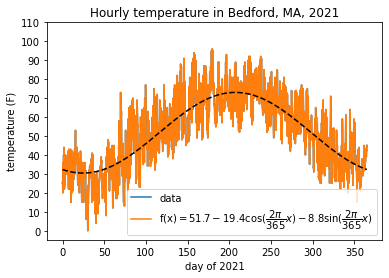
\includegraphics[width=0.45\linewidth]{img/C03weatherBedfordfit.png}
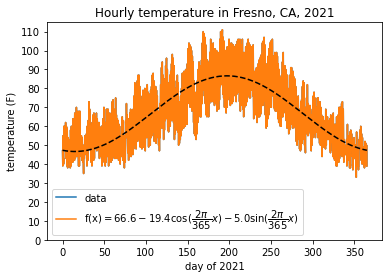
\includegraphics[width=0.45\linewidth]{img/C03weatherFresnofit.png}



\subsection{Normal equations}

See the text for a geometric explanation of how these equations solve the linear least squares problem.

\begin{enumerate}[resume]
    \item Given a dataset with $m$ pairs, and a model with $n$ parameters, identify the dimensions of $A^TA$, $\mathbf{c}$, and $A^T\mathbf{y}$.    
\end{enumerate}

\section{Error due to approximations}

\subsection{Forward and backward error}

Consider a function $f(x)$.  Set $y = f(x)$.

In a computer, even if $x$ is exact, approximations occur during the calculation steps of the function, so the computed value is $\hat{y}$ instead of $y$.

The computed value would be the exact solution for a slightly different input, $x + \Delta x$.




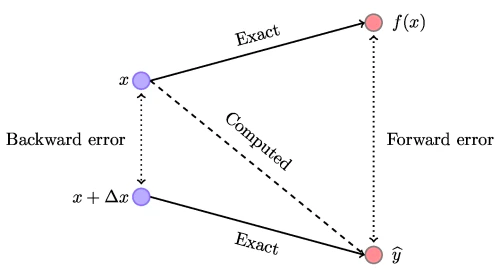
\includegraphics[scale=0.6]{img/C01errorNickHingham.png}

\href{https://nhigham.com/2020/03/25/what-is-backward-error/}{Image from Nick Higham's blog}



\vspace{0.2cm}
\hrule
\vspace{0.2cm}

\noindent \textbf{Definitions: error}

\begin{tcolorbox}
\begin{itemize}
\itemsep0pt
\item \textbf{Forward error} refers to the error in the output a process.  It is given by $\left\vert y - \hat{y}\right\vert$ (\textbf{absolute}) or $\left\vert \dfrac{y - \hat{y}}{y}\right\vert$ (\textbf{relative}).
\item \textbf{Backward error} refers to the difference between the true input and the apparent input, and is given by $\left\vert x - \hat{x}\right\vert$ (\textbf{absolute}) or $\left\vert \dfrac{x - \hat{x}}{x}\right\vert$ (\textbf{relative}).
\item The error magnification factor is the ratio of the two: 

$\text{error magnification factor} = \dfrac{\text{relative forward error}}{\text{relative backward error}}$.  This is also referred to as the \textbf{condition number} for the problem.

\item If either $x$ or $y$ is close to zero then the condition number may be calculated using absolute error: $\text{cond } \#=\dfrac{\left\vert (y - \hat{y})\right\vert}{\left\vert (x - \hat{x})\right\vert}$

\item The matrix \textbf{condition number} is the maximum possible error magnification factor.


\end{itemize}
\end{tcolorbox}


\vspace{0.2cm}
\hrule
\vspace{0.2cm}

\noindent \textbf{Condition number}
\begin{enumerate}[resume]
\item
Consider $y = f(x)$ for some function $f$.  If the condition number is $\approx 1$, and you change your input value by $1\%$, how do you expect the output value to change?

\vspace{0.5in}

\item
What if the condition number is $100$?  In this case, if you change your input value by $1\%$, how do you expect the output value to change?

\vspace{0.5in}
\end{enumerate}

\begin{tcolorbox}
\begin{itemize}
\itemsep0pt
\item A problem is \textbf{well conditioned} when small changes in the input lead to comparably small changes in the output.

\item A problem is \textbf{ill conditioned} when the output is sensitive to small changes in the input (or the reverse).
\end{itemize}

\end{tcolorbox}

We will be vague about the exact threshold for well- vs ill- conditioned.

\subsection{Normal equations and conditioning}

For the normal equations, we are solving $A^TA\overline{\mathbf{c}} = A^T\mathbf{y}$ for $\overline{\mathbf{c}}$, so the output of our calculation is $\overline{\mathbf{c}}$.

For solving $A\mathbf{x} = \mathbf{b}$ for $\mathbf{x}$ (so $\mathbf{b}$ is the input and $\mathbf{x}$ is the output), the \textbf{condition number} for matrix inversion, $\text{cond}(A)$, tells us about the maximum error magnification for this problem.

$\text{cond}(A^TA) = \text{cond}(A)^2$, so using the normal equations the maximum error is squared compared to the condition number for $A$.

This makes the normal equations especially vulnerable to magnifying numerical error.


Note: we will treat matrix condition number as a black box.  There is a way to calculate, it, but we will not discuss that right now.

\end{document}